\chapter{Versioning approaches}
\label{chap:versioning-approaches}

The service API can be versioned in multiple ways. One of the approaches is deployment of new version to new environment. This approach is widely used for code versioning not only for services. The other approach is specific for services. Multiple versions can coexist at the same time. Then a question arises of how a consumer can access the requested version of the service. The possibilities of accessing them are analyzed in chapter \ref{chap:versionaccess}.


\section{Universal versioning approach}
The versioning is based on deploying a new version of \gls{api} to a new environment. The versioning approach is identical to software deployment. Service changes are deployed on a new environment which has its unique URL address. 


A client has the production environment with a version of API. When the changes are done to this API and it's created a new version, client has to integrate the changes. If there is only one production environment the new version is deployed and it replaces the old one. In case, there are more environments available both version can be available while each of the environments has its specific URL address, this is shown on figure \ref{fig:universal-versioning}. When the client calls the particular API version there is no need to mention its version in URL.


\begin{figure}[htp] \centering{
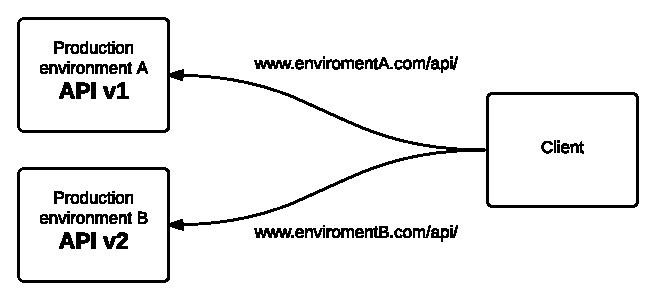
\includegraphics[width=9cm]{img/universal-versioning.pdf}}
\caption{Universal versioning approach - possibility of access two versions}
\label{fig:universal-versioning}
\end{figure} 


\section{Services specific versioning}
Another approach to versioning is more than one version of the service API running at the same time. This approach can be implemented using various principles. \emph{Services versioning} brings the challenge to access the requested version. Version access approaches will be explained in chapter \ref{chap:versionaccess}.


This versioning approach allows to make changes to the API and release its new version without waiting for consumers to integrate the changes. All versions can run concurrently and be accessed by clients. When there are two coexistent versions of API, \emph{v1} and \emph{v2}, consumer has access to both of them. According to what was sent in the request, consumer is directed to the correct version (figure \ref{fig:services-specific-versioning}). Each of these versions can be on the same environment, or can be separated. This concept is invisible to consumers.


\begin{figure}[htp] \centering{
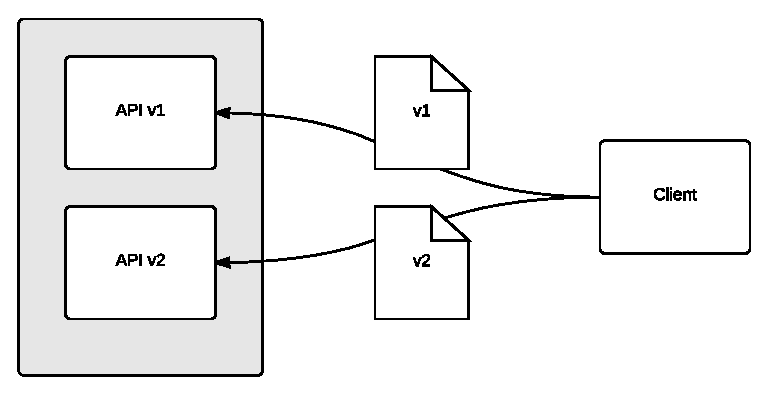
\includegraphics[width=9cm]{img/services-specific-versioning.pdf}}
\caption{Services versioning approach - the version is specified in requests}
\label{fig:services-specific-versioning}
\end{figure} 


\subsection{Units of versioning}
\label{sec:units}
The service layer of an application developed by a provider is an \emph{API} containing \emph{services}. Services contain \emph{methods (actions)} which allow to manipulate with the resources. The relationship between these entities is shown on figure \ref{fig:service-layer-design}

\begin{figure}[htp] \centering{
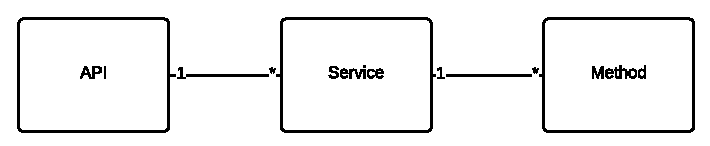
\includegraphics[width=11cm]{img/service-layer-design.pdf}}
\caption{Design of service layer}
\label{fig:service-layer-design}
\end{figure} 

Having this hierarchy there are three possibilities of what can be versioned in service interface. The granularity of versioning can be defined by the change which caused the creation of new version. If the change happens in method it is possible to version only the method. On the other hand, when a set of services are changed, whole API can be versioned. These are not rules but decisions. What to version should originate from the versioning strategy. 


Version is usually identified by one digit. This applies for each of the version unit. Than the architecture with different version of API, service and method can looks like the example on figure \ref{fig:version-unit}. The versioning on levels of API is shown there. The second part is a service versioning, \emph{Orders} service has two versions within an API. Third part shows versioned method \emph{Get} which has \emph{v1} and \emph{v2} implementations.


\begin{figure}[htp] \centering{
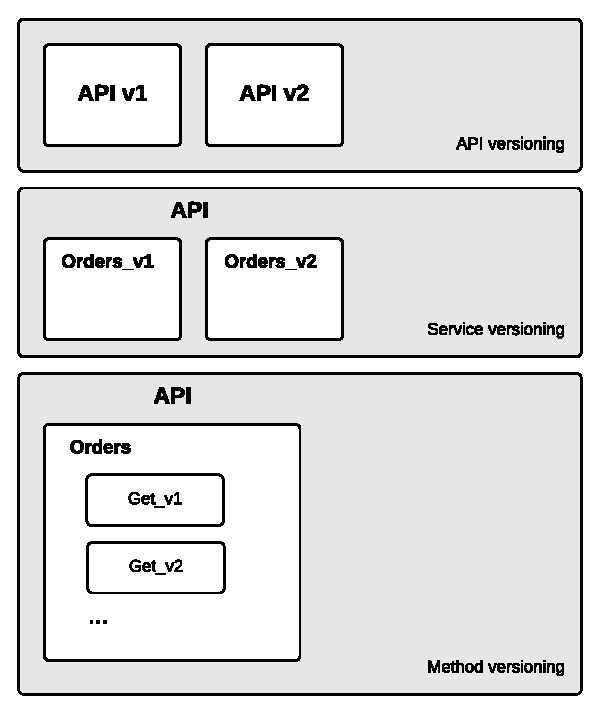
\includegraphics[width=9cm]{img/version-unit.pdf}}
\caption{Versioning units}
\label{fig:version-unit}
\end{figure} 


The three options can be combined. However combination of versioning of different granularity can result in complicated architecture of provided services.


\begin{description}
\item{API versioning} \\
The API containing all services can be versioned. Having a version \emph{v1} API is incremented to version \emph{v2}. This new version can be deployed on the same environment which was running the API \emph{v1}. Consumers can access them both. Main disadvantage is the amount of redeployed code which contains mostly duplicated unchanged part of services. 
\item{Service versioning} \\
  A whole service is versioned with all its methods. Versioned service with version \emph{v1} is changed to \emph{v2}. It is still part of the API \emph{v1}, just the service version is incremented. When the new version on the service is deployed on an environment, both service versions can be accessed. 
\item{Method versioning} \\
  In most cases the change arises just in a method or a few methods of a service. It is not necessary to version the whole service, but there is an option to version just these methods. 
  
  Benefits of this approach are:
  
  \begin{enumerate}
    \item It minimizes the amount of deployed code. Only changed methods are redeployed in a new version
    \item It allows immutable services names. There are only addition of new method or method deprecations.
  \end{enumerate}
  
  However it has this disadvantages:
  
  \begin{enumerate}
    \item It requires more complex addressing schema. Instead of calling only service, consumers have to specify also the method and version of method which want to use.
    \item Versioned methods have to be deployed independently. Moreover every method has its own endpoint address.
  \end{enumerate}
\end{description}


\subsection{Logic of service versioning}
There is a version of an API which is being used in production. A breaking change needs to be applied and new API version is created. Both versions can be deployed into production, it is not mandatory for both of them to be on the same environment but they have the same \gls{domain-name}. Consumer can continue to use the old version, he can switch to new version integrating the changes when he decides to. It is needed to be clear in advance about how will it be accessed.

Depending on the principle of accessing the version, it can be said explicitly in endpoint address (URL) which version of API, service or method is called. The request is directly roated to requested version. The other approach is to have the same endpoint address for each version of the versioned unit. Routing passes through an intermedia which resolves the correct version. Decision is based on one of the parameters sent in request. Ways of accessing the version will be described in chapter \ref{chap:versionaccess}.


\section{Comparison of analyzed versioning approaches}
Both of described service versioning principles have their advantages. Some of them are summarized within this section. 

\begin{enumerate}
  \item {Error fixes} \\
The main disadvantage of first approach but also the API versioning of the second one is the incapability of easily repair issues in a previous version of the API. When the API is in versions up to \emph{v3} in development environment and in versions \emph{v1} and \emph{v2} in production environment. When an error is found in production in \emph{v1} (figure \ref{fig:bug-in-previous-version}) this bug is probably present also in later versions - \emph{v2} and \emph{v3}. Then the bug has to be fixed in all three versions and redeployed on servers, which is usually not a trivial operation.
\begin{figure}[htp] \centering{
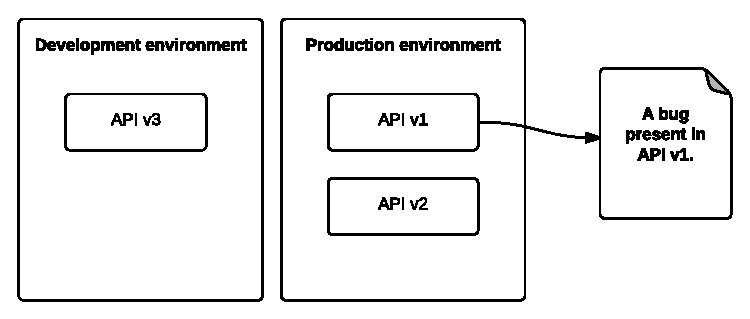
\includegraphics[width=11cm]{img/bug-in-previous-version.pdf}}
\caption{An error found in one of the previous version}
\label{fig:bug-in-previous-version}
\end{figure} 

When the service versioning is made on the service or method level, the bug fixes are easier because the different version shares parts of the code. If an error is present in this shared code, then the fix is required only in one place.


\item{Number of accessible versions} \\
In case of having universal versioning principle and client needs to have access to both versions, he's forced to have two production environments. Than the costs of the application are increasing, because of high prices of production environments and maintenance of both consumed APIs. The services principle offers more than one version accessible at the same time


\item{Version accessibility} \\
The advantage of universal approach is access to the API. There is only one stable address to one version. Regarding to the services versioning more versions coexist and client has to specify which he wants to access. Client is forced to add the version identification in the requests, he has to change it everytime he change the version of API or its subunits. For provider it is needed to implement a logic of accessing different versions.

\end{enumerate}




